\documentclass[12pt]{article}
\usepackage[utf8]{inputenc}
\usepackage[ngerman]{babel}
\renewcommand\thesection{\arabic{section}}
\usepackage{graphicx}
\usepackage{amsmath}
\usepackage{amsfonts}
\usepackage{amssymb}
\usepackage{dsfont }
\usepackage{color}
\usepackage{hyperref}
\usepackage{subfigure}
\usepackage{wrapfig}

\title{Statistical learning Seminar\\Berlin airbnb: Analyse und Angebotpreisvorhersage }
\author{Minh Anh Le - Leander Piepenbring  }
\date{Wirtschaftsmathematik - HTW Berlin\\\\Februar 2022 }

\begin{document}
\setcounter{tocdepth}{1}
\newpage
\maketitle
\newpage
\tableofcontents
\newpage
\listoffigures   
\newpage
\part{Einleitung}
\section{Motivation}
\begin{text}

Seit einigen Jahren gehen die Immobilienpreise, und somit auch die Mieten steil nach oben. Besonders stark sind davon große Städte betroffen. Viele Leute möchten deshalb in der Zeit, in der sie nicht vor Ort sind, ihre Wohnung (unter)vermieten.
\\\\
\begin{wrapfigure}{l}[0pt]{0.5\linewidth}

\includegraphics[width=0.3\textwidth]{airbnb_lockup_web.png}
\end{wrapfigure}
An dieser Stelle kommt Airbnb in Spiel. Airbnb ist ein Online-Wohnungsportal, das den Benutzern ermöglicht, ihre eigenen Wohnungen anzubieten, andere Angebote zu entdecken und Buchungen abzuschließen. Airbnb finanziert sich dabei über eine Gebühr von 3 Prozent pro Buchung und weitere kleine Service-Gebühren.
\\\\
Dieses Projekt zielt darauf ab, die Immobilienpreisentwicklung in Berlin anhand eines Airbnb-Datensatzes nachzuvollziehen. Dabei werden unterschiedliche Fragestellungen betrachtet und diese anhand von deskriptiven Analyse-Methoden beantworten.
\\\\
Ein weiteres Ziel dieses Projektes ist, einen Preis für ein gegebenes Angebot vorherzusagen und die Merkmale zu filtern, die den Preis am stärksten beeinflussen. Dafür wird die Random Forest Methode angewandt.




\newpage
\part{Datenanalyse}
\section{Explorative Datenanalyse} 
\subsection{Abrufen der Daten}
Die Daten, die für dieses Projekt verwendet werden, kommen von InsideAirbnb. InsideAirbnb ist eine unabhängige Internetseite, auf der man detaillierte Informationen über Airbnb Angebote auf der ganzen Welt erhalten kann. InsideAirbnb nimmt seine Daten dabei direkt von der Airbnb Website. Die Daten werden für alle  Städte separat zur Verfügung gestellt.
\\\\
Die Daten umfassen eine Fülle an Informationen über die Angebote, wie den Preis pro Nacht, die Anzahl der Gäste, die Verfügbarkeit der Unterkunft, die Lage und vieles weitere.
\\\\
Für dieses Projekt wurde der Listings Datensatz und der Calendar Datensatz verwendet. Die Daten umfassen den Zeitraum vom 22.09.2021, bis zum 21.09.2022 und wurden am 05.12.2021 für dieses Projekt heruntergeladen.

\newpage
\subsection{Listings Datensatz}
Der Listings Datensatz umfasst insgesamt 18288 Angebote und es gibt 74 verschiedene Merkmale. Aufgrund der hohen Anzahl an Merkmalen, werden für dieses Projekt nur Merkmale berücksichtigt, von denen erwartet wird, dass sie einen signifikanten Einfluss auf die Preisbildung haben.


\begin{figure}[h]
 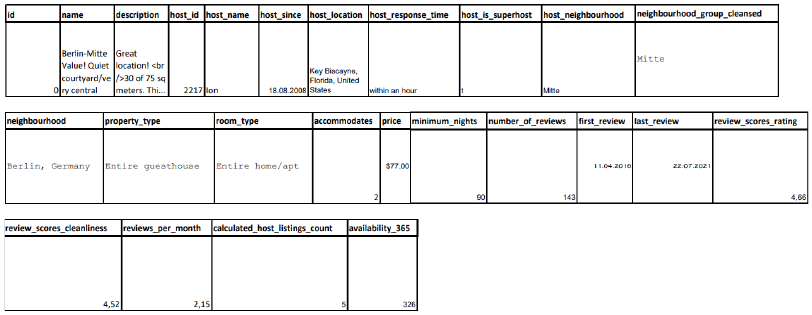
\includegraphics[width=1\textwidth]{ListingTabelleNeu.png}
 \caption{Beispiel Datensatz aus Listings}
\end{figure}
\\
\begin{itemize}
    \item \textbf{ID}: Das Kennzeichen des Angebotes.
    \item \textbf{Name}: Der Titel des Angebotes.
    \item \textbf{Description}: Kurze Beschreibung über das Angebot. 
    \item \textbf{Host ID}: Das Kennzeichen des Vermieters.
    \item \textbf{Host name}: Der Name des Vermieters.
    \item \textbf{Host since}: Der Tag, am dem der Vermieter das Konto bei airbnb eröffnet hat.
    \item \textbf{Host location}: Der aktuelle Ort von dem Vermieter 
    \item \textbf{Host response time}: Wie schnell Anfragen vom Host beantwortet werden
    \item \textbf{Host ist superhost}: Status des Vermieters, ob er Superhost ist. \\ (t oder f)
    \item \textbf{Host neighbourhood}: Stadtteil, in dem der Host wohnt
    \item \textbf{Neighbourhood group cleansed}: Der Stadteil des Angebotes
    \item \textbf{Neighbourhood}: Die Stadt des Angebotes
    \item \textbf{Property type}: Angaben, über die Immobilie 
    \item \textbf{Room type}: Angaben über Räumlichkeiten
    \item \textbf{Accomodate}: Die Anzahl der Gäste, die zu dem Angebot passt.
    \item \textbf{Price}: Der Preis pro Nacht (angegeben in USD)
    \item \textbf{Minimum nights}: Mindestanzahl an Nächten
    \item \textbf{Number of reviews}: Anzahl der Reviews
    \item \textbf{First review}: Datum des ersten Reviews
    \item \textbf{Last review}: Datum des letzten Reviews
    \item \textbf{Review score rating}: Gesamtbewertung des Angebots (0 - 5)
    \item \textbf{Review score cleanliness}:Bewertung der Sauberkeit (0 - 5)
    \item \textbf{Review per month}: Anzahl der Reviews pro Monat
    \item \textbf{Calculated host listings count}: Anzahl der Angebote des Hosts.
    \item \textbf{Availability 365 }: Anzahl der Tage, die das Angebot verfügbar ist pro Jahr.
    
    
\end{itemize}

\newpage
\subsection{Calendar Datensatz}
Der Calendar Datensatz gibt Auskunft darüber, ob ein Angebot für jedes Datum zwischen dem 22.09.2021 und dem 21.09.2022 verfügbar (t) oder nicht Verfügbar (f) ist. Für jedes Angebot gibt es also 365 Datensätze, wodurch der Calendarsatz insgesamt 6674848 Datensätze umfasst. Der Datensatz ist in 7 verschiedene Merkmale unterteilt.


\begin{figure}[h]
 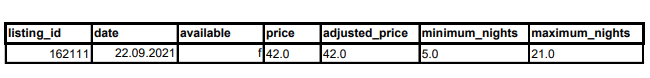
\includegraphics[width=1\textwidth]{CalendarTabelleNeu.png}
 \caption{Beispiel Datensatz aus Listings}
\end{figure}

\begin{itemize}
    \item \textbf{Listing ID}: Eindeutiges Kennzeichen des Angebots
    \item \textbf{Date}: Datum TT.MM.JJJJ
    \item \textbf{Availability}: Verfügbarkeit des Angebots zu jedem Tag des Jahres \\ (t oder f)
    \item \textbf{Price}: Preis pro Nacht
    \item \textbf{Adjusted Price}: Angepasster Preis
    \item \textbf{Minimum Nights}: Mindestanzahl an Nächten
    \item \textbf{Maximum Nights}: Maximalanzahl an Nächten
\end{itemize}

\newpage
\part{Methodik und Modellierung}

Um den Preis pro Nacht vorherzusagen und die Merkmale zu filtern, die den Preis am meisten beeinflussen wurden Modelle des Machine Learning verwendet. Diese Algorithmen verwenden die Daten und verschiedene Annahmen, um die Ausgabevariable, den Preis pro Nacht eines Airbnb Angebots vorherzusagen. Der Datensatz wurde in ein 70/30 Train-Set und Test-Set aufgeteilt. Diese Stichproben wurden in Random Forest-Modelle implementiert, um ihre Leistungsmetriken in das Bestimmtheitmaß $R^2$ , die mittlere quadratische Abweichung (MSE), den mittlereren absoluten Fehler (MAE) und die Wurzel der mittleren Fehlerquadratsumme (RMSE) zu bewerten.

\section{Random Forest}
\subsection{Definition}
        \underline{Was ist Random Forest?}\\\\
Der Random Forest Algorithmus ist ein überwachter Lernalgorithmus, der für Klassifizierungs- oder Regressionsaufgaben verwendet wird. Er wird sehr gerne verwendet, weil nur wenige Annahmen über die Verteilung der Daten getroffen werden müssen und die Ergebnisse trotzdem sehr zufriedenstellend sind. Diese Methode wird wegen ihrer guten Vorhersagekraft, hohen Interpretierbarkeit und Gewichtung der wichtigsten Merkmale verwendet.
\\
\subsection{Funktionalität}\\
    \underline{Wie funktioniert Random Forest?}\\\\
Der Random-Forest-Algorithmus stellt Regeln bereit, wie viele verschiedene Entscheidungsbäume generiert werden, die dann mithilfe einer speziellen Ensemble-Methode kombiniert werden, um ein Ergebnis zu erzeugen. Beim Erstellen dieser Entscheidungsbäume wird jedes Mal, wenn eine Teilung in einem Baum betrachtet wird, eine Zufallsstichprobe von m Prädiktoren als Teilungskandidaten aus dem vollständigen Satz von p Prädiktoren ausgewählt. Die Aufteilung darf nur einen dieser m Prädiktoren verwenden. Normalerweise wird $m \approx \sqrt{p}$ verwendet, das bedeutet, dass die Anzahl der bei jeder Teilung berücksichtigten Prädiktoren ungefähr gleich der Quadratwurzel der Gesamtzahl der Prädiktoren ist. Das Ziel des Projektes war es, den Random Forest Algorithmus zu verwenden, um den Preis eines Angebots pro Nacht in Berlin  basierend auf den 51 Merkmalen mit der größten Varianz im Trainingsset vorherzusagen. Der gesamte Datensatz wird zufällig in einen Trainings- und einen Testsatz aufgeteilt und Random Forest auf den Trainingssatz für drei verschiedene Werte der Anzahl der Teilungsvariablen m angewendet. Die Ergebnisse sind in Abbildung 8 dargestellt. Die bestmögliche Wahl für m und p sind m = 40 und p = 200.
\\
\section{Entscheidungsbaum}
\subsection{Definition}
        \underline{Was ist ein Entscheidungsbaum?}\\\\
Ein Entscheidungsbaum ist eine grafische Darstellung der möglichen Ergebnisse oder Auswirkungen einer Reihe verwandter Entscheidungen. Dieser Ansatz ermöglicht die Klassifizierung oder Regression einer großen Anzahl unterschiedlicher Datensätze und kann zur Entwicklung mathematischer Algorithmen zur Vorhersage der besten Wahl verwendet werden.
\subsection{Funktionalität}\\
    \underline{Wie funktioniert Entscheidungbaum?}\\\\
Entscheidungsbäume beginnen typischerweise mit einem einzelnen Knoten, aus dem Zweige hervorgehen, die die entsprechenden Ergebnisse verwandter Entscheidungen darstellen. Jedes Ergebnis ist mit anderen Knoten verbunden, die wiederum andere potenzielle Auswirkungen haben.  \\
Die Knoten haben zwei Möglichkeiten:
\begin{itemize}
    \item Bedingungen [Entscheidungsknoten]
    \item Ergebnis [Endknoten]
\end{itemize}
Die Kanten stellen die Wahrheit oder Falschheit einer Aussage dar, und eine Entscheidung wird basierend auf dem folgenden Beispiel getroffen, das einen Entscheidungsbaum zeigt, der die größte von drei Zahlen auswertet.
\begin{figure}[h]
\begin{center}
 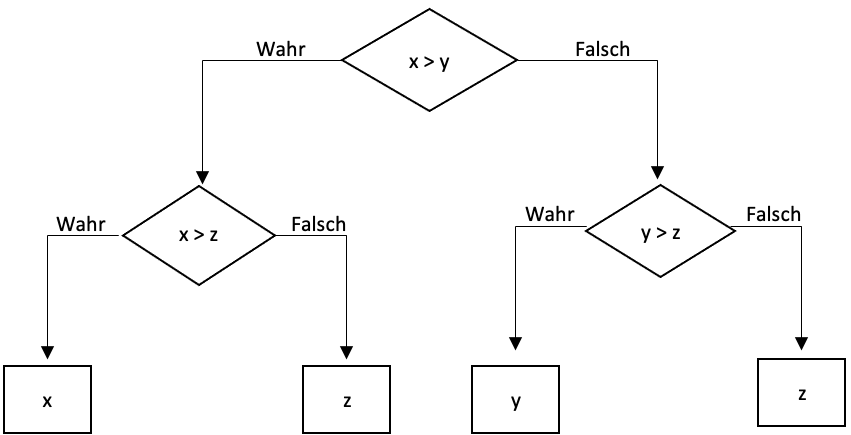
\includegraphics[width=0.8\textwidth]{entscheidungsbaum .png}
 \caption{Beispiel Entscheidungsbaum}
\end{center}
\end{figure}
\\\\
\section{Modellierung}
Bevor der Random Forest Algorithmus angewendet werden kann, müssen die Merkmale mit Datentyp \textbf{String} oder \textbf{Object} zu \textbf{float}, \textbf{integer}, \textbf{boolean} oder \textbf{array} umgewandelt werden. Danach werden die Daten in zwei verschiedene Sets aufgeteilt: Training Set und Test Set, enthält jeweils einen Vektor Y und eine Matrix X: 
\begin{itemize}
    \item der Vektor Y, der alle realen Preise des Datensatzes enthält
    \item die Matrix X, die alle Merkmale enthält, die für den Preis relevant sind
\end{itemize}
\newpage
Um einen Overfit dieses Modells zu vermeiden, wird ein Tool von sklearn verwendet, um die Beobachtungen in zufälligen Training-Set und Test-Set aufzuteilen:
\\
\begin{figure}[ht]
\begin{center}
 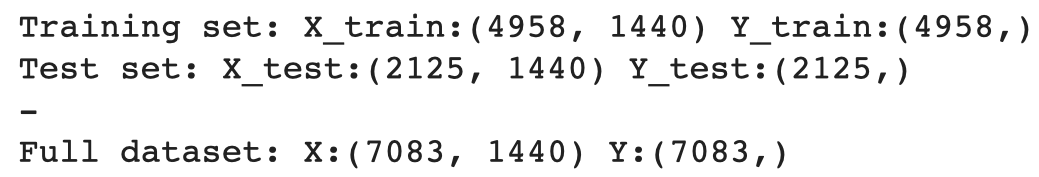
\includegraphics[width=0.8\textwidth]{split_Set.png}
 \caption{Train-,Test-Set Übersicht}
\end{center}
\end{figure}
\\
Danach wird Random Forest auf den Trainingssatz für drei verschiedene Werte der Anzahl der Teilungsvariablen m = max\_depth und den Wert der Gesamtsbäume p = n\_estimators angewendet. 
\\\\
m entspricht der Anzahl der Merkmale, die durchlaufen werden und p der Anzahl der Entscheidungsbäume, die generiert werden sollen.
\\\\
Als Beispiele werden n = 20, n = 35 und n = 40 genommen. Für die Anzahl der Bäume wird p = 200 verwendet.
\\\\
Ergebnis in Abbildung 9.


\newpage
\part{Visualisierung}
\section{Deskriptive Analyse}
Um einen Überblick über den Berliner Airbnb-Wohnungsmarkt zu bekommen werden im folgenden einige datenspezifische Fragen anhand deskriptiver Analysemethoden beantwortet.
\\\\
\underline{Wo gibt es die meisten Angebote in Berlin?}

\begin{figure}[h]
 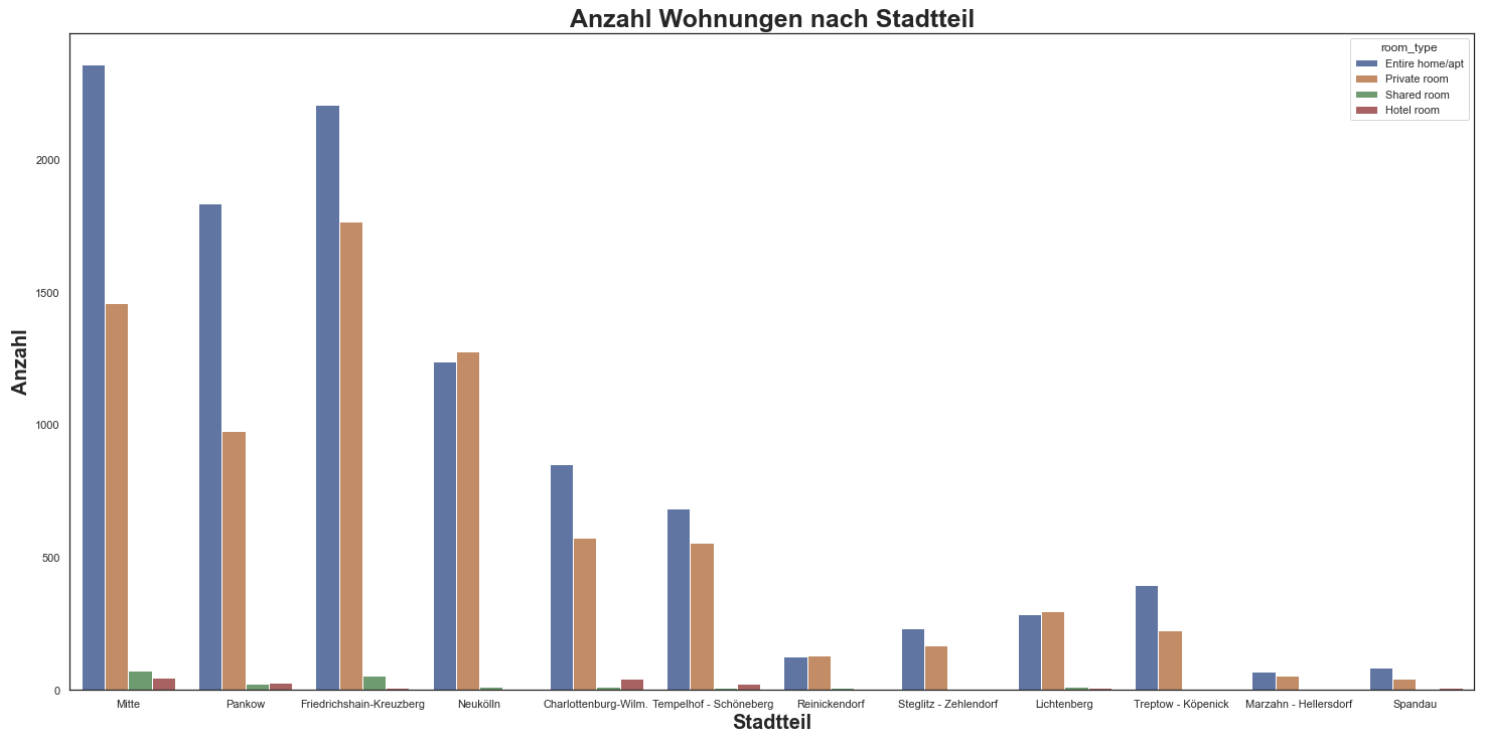
\includegraphics[width=1.1\textwidth]{AnzahlBild.PNG}
 \caption{Anzahl Wohnungen nach Stadtteil}
\end{figure}

In dieser Grafik werden die Anzahl der Wohnungen nach Stadtteil und Wohnungsart dargestellt. Es lässt sich leicht erkennen, dass die Stadtteile mit den meisten Angeboten Mitte, Kreuzberg, Pankow und Neukölln sind. Diese Verteilung ist wahrscheinlich darauf zurückzuführen, dass diese Stadtteile sehr zentral liegen und sich dadurch gut für einen Urlaub in Berlin eignen. 
\\\\
Außerdem können wir der Grafik entnehmen, dass es vier verschiedene Wohnungsarten gibt (private Zimmer, geteilte Zimmer, Wohnungen/Häuser, Hotelzimmer) und es in Berlin hauptsächlich Angebote füt private Zimmer und Wohnungen/Häuser gibt. Das Angebot für geteilte - und Hotelzimmer ist sehr gering. In manchen Stadtteilen, wie zum Beispiel Marzahn-Hellersdorf oder Treptow-Köpenick gibt es gar keine Angbote für diese Wohnungsarten.
\\\\
\underline{Wie verteilt sich der Preis nach Wohnungsart?}
\\\\
Nun soll veranschaulicht werden, wie sich der Preis pro Nacht innerhalb der einzelnen Wohnungsarten verteilt.
\begin{figure}[h]
 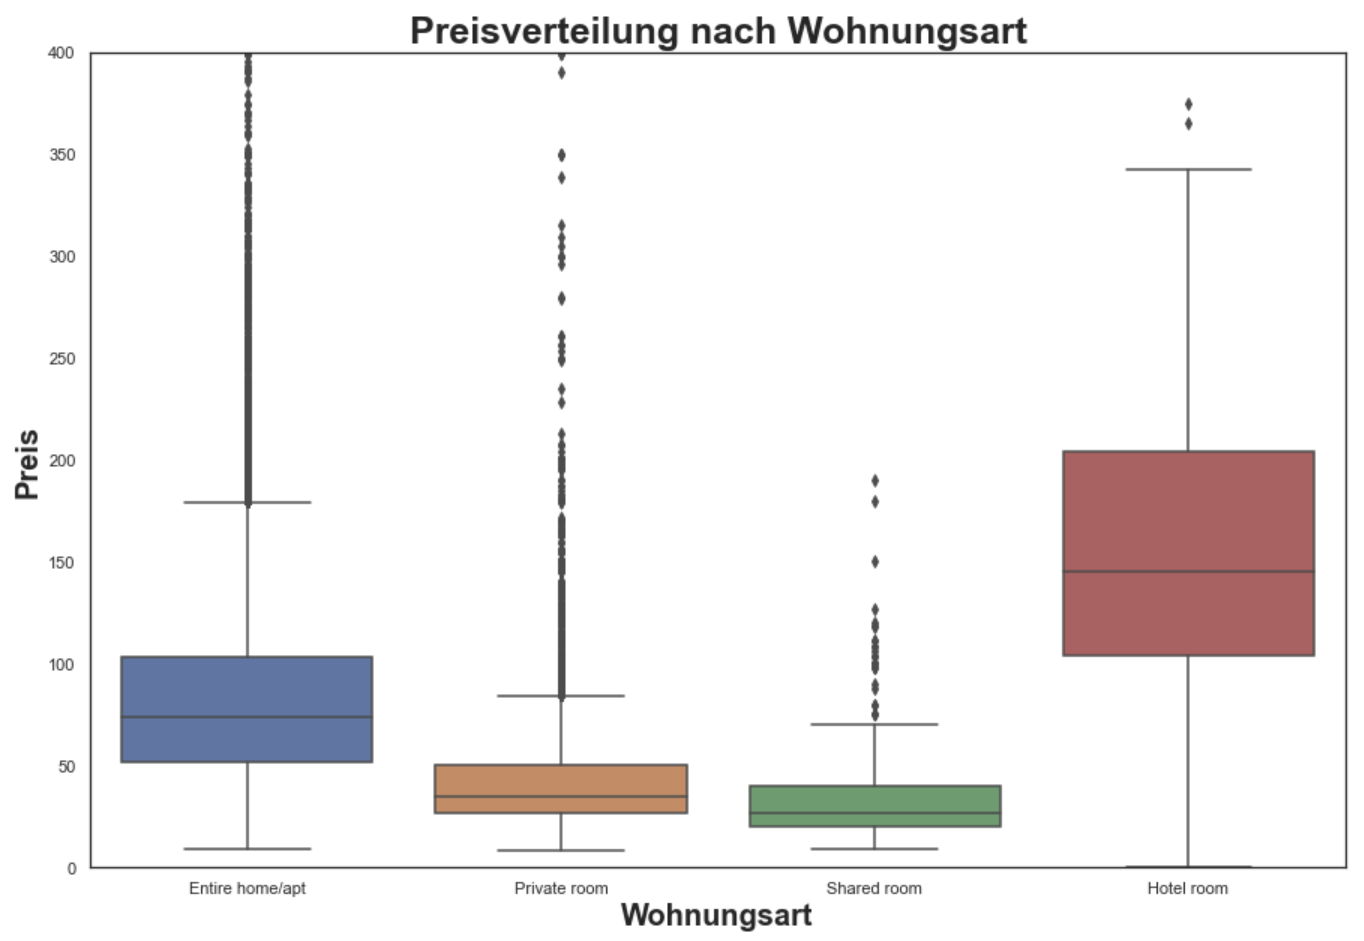
\includegraphics[width=1.1\textwidth]{RoomTypeBild.PNG}
 \caption{Preisverteilung nach Wohnungskategorie}
\end{figure}

\newpage
Zunächst soll die Kategorie "Wohnungen/Häuser" betrachtet werden. 
\\
Der Median für diese Wohnungsart liegt bei 74\$ pro Nacht. Es liegen also die Hälfte der Angebote über und die andere Hälfte unter dem Wert von 74\$ pro Nacht. Ein Viertel der Angebote hat einen geringeren Preis als 52\$ und ein Viertel einen höheren Preis als 103\$ pro Nacht. Es liegt also die Hälfte der Angebote zwischen 52\$ und 103\$ pro Nacht. Es fällt allerdings auf, dass es nach oben sehr viele Ausreißer gibt. Diese reichen bis zu einem Preis von 1000\$ pro Nacht.
\\\\
Die nächste zu betrachtende Kategorie ist "Private Zimmer". 
\\
In dieser Wohnunsart liegt der Median bei 35\$ pro Nacht. Die Hälfte der Angebote liegt zwischen 27\$ und 50\$ pro Nacht. Auch in dieser Kategorie fällt, auf , dass es nach oben sehr viele Ausreißer gibt.
\\\\
Nun zur Kategorie "Geteilte Zimmer".
\\
Der Median liegt bei 27\$ und der Interquartilsabstand befindet im Bereich von 20 - 40\$. Der Großteil der Ausreißer bei dieser Wohnungsart erstreckt sich bis zu einem Preis von 200\$ pro Nacht. Bei dieser Wohnungsart handelt es sich also um die günstigste Kategorie.
\\\\
Die letzte Kategorie bildet die Wohnungsart "Hotel Zimmer".
\\
Der Median liegt hier bei 147\$ und ist damit deutlich höher als bei den vorherigen Kategorien. Der Interquartilsabstand erstreckt sich von 105\$ bis 205\$. Im Vergleich zu Kategorie 1 und 2 weist die Wohnungsart "Hotel Zimmer" deutlich weniger Ausreißer nach oben auf. Dies kann auf die seriöse Preisgestaltung von Hotels zurückgeführt werden.
\\\\

\newpage
\underline{Wie verteilt sich der Preis innerhalb der Stadtteile?}
\\\\
Da es für die Kategorien Geteilte - und Hotelzimmer nur sehr wenige Angebote gibt, werden in der folgenden Grafik lediglich die Kategorien Häuser/Wohnungen und Private Zimmer betrachtet.

\begin{figure}[h]
 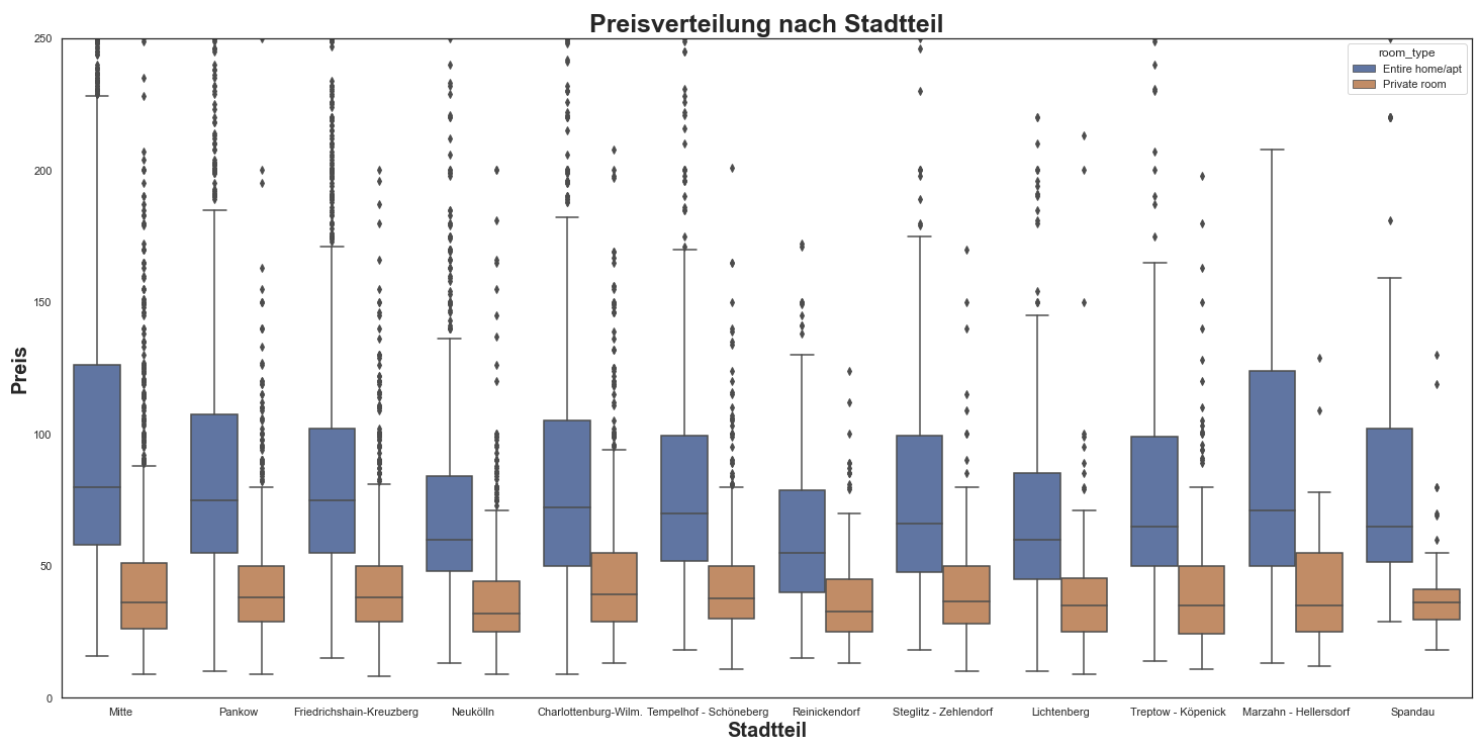
\includegraphics[width=1.1\textwidth]{StadtteileBild.PNG}
 \caption{Preisverteilung nach Stadtteil}
\end{figure}

Auf den ersten Blick sieht man, dass die Mediane der verschiedenen Stadtteile sehr nahe beieinander liegen. Auf den zweiten Blick lassen sich aber durchaus unterschiede in der Länge der Whisker und der Anzahl der Ausreißer erkennen. Als Beispiel wird im Folgenden der Unterschied zwischen Spandau und Mitte betrachtet.
\\
In der Kategorie Häuser/Wohnungen liegt der Median von Mitte leicht über dem von Spandau. Die Länge des oberen Whiskers beträgt bei Mitte 100, während sie bei Spandau nur 57 beträgt und damit fast halb so lang wie bei Mitte. Außerdem gibt es in Mitte eine sehr große Häufung von Ausreißern, während es bei Spandau nur sehr wenige sind. Ein ähnliches Resultat lässt sich auch bei den Privaten Zimmern feststellen.
\\
In Mitte gibt es allerdings auch günstigere Angebote als in Spandau, was man an der Länge des unteren Whiskers erkennen kann. Dies liegt daran, dass es in Mitte eine beträchtliche Anzahl an Angeboten gibt. (Siehe Abbildung 5)
\\\\
Man kann also festhalten, dass die Bezirke Mitte, Pankow, Friedrichshain-Kreuzberg und Charlottenburg-Wilm. eher der höherpreisigen Kategorie anzuordnen sind und Spandau bzw. Reinickendorf eher im niedrigeren Preissegment zu finden sind.
\\\\
\underline{Wie entwickelt sich der Preis im Verlauf der Woche?}

\begin{figure}[h]
 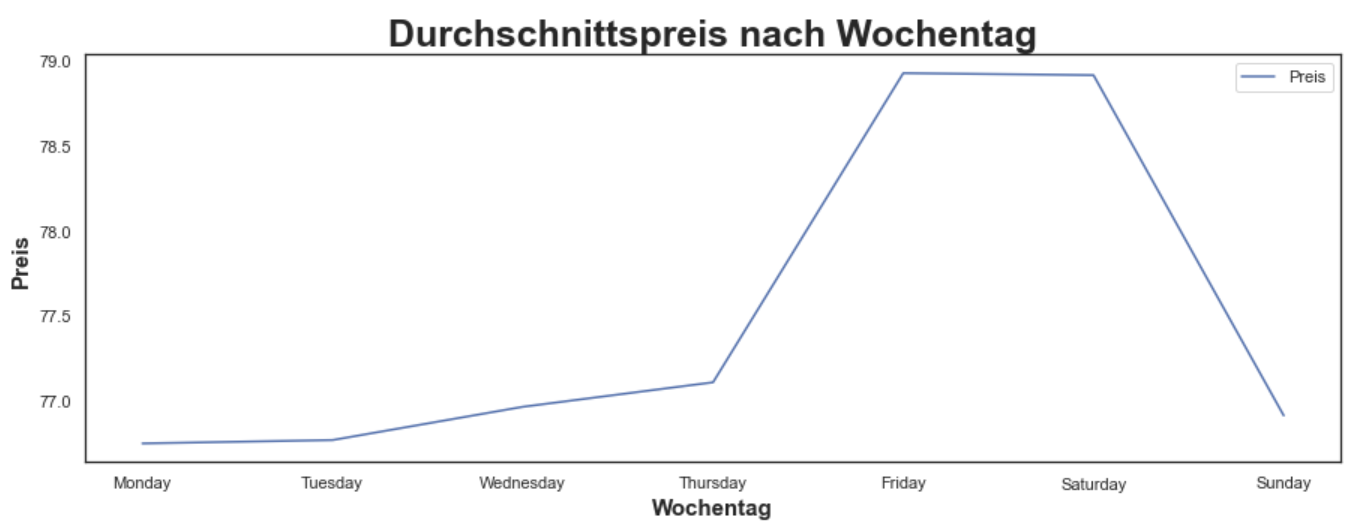
\includegraphics[width=1.1\textwidth]{WochePreisBild.PNG}
 \caption{Preisentwicklung über die Woche}
\end{figure}

Wie man unschwer der Grafik entnehmen kann, gibt es einen leichten Anstieg im Durchschnittspreis am Wochenende. An den tagen Montag und Dienstag liegt der Durchschnittspreis bei 76,75\$ und steigt im Verlauf der Woche bis 78,9\$ an. 
\\
Dies liegt offensichtlich daran, dass die Nachfrage an verfügbaren Angeboten am Wochenende ansteigt.

\newpage
\part{Empirische Ergebnisse}
Vier Hauptmetriken, anhand derer die Modelle bewertet wurden, waren das Bestimmtheitmaß $R^2$ ,die mittlere quadratische Abweichung (MSE), der mittlerer absoluter Fehler(MAE) und der Wurzel der mittleren Fehlerquadratsumme Fehler (RMSE).
\\\\
Der $R^2$ Wert ist ein statistisches Maß für den Anteil der Variabilität in der vorhergesagten Variablen, die durch das Regressionsmodell erklärt wird.
\begin{center}
    $R^2 = 1- \frac{\sum{(y_i-\hat{y})^2}}{\sum{(y_i-\bar{y})^2}}$
\end{center}
\\\\
Der RMSE Fehler misst die Standardabweichung der Residuen um die angepasste Regressionslinie.
\begin{center}
    $RMSE= \sqrt{MSE} = \sqrt{{\frac{1}{n}}\sum\limits_{t=1}^{n}{(y_i-\hat{y})^2}}$
\end{center}
\\\\
Der mittlerer absoluter Fehler (MAE) wird verwendet, um die Genauigkeit von Vorhersagen bestimmen.
\begin{center}
    $MAE = \frac{1}{n}\sum\limits_{i=1}^{n}{|\hat{y_i}-y_i|}$
\end{center}
wobei folgende Variablen Verwendung finden:
\begin{itemize}
    \item n: Anzahl der Vorhersagewerte
    \item $\hat{y_i}$: Vorhersagewerte
    \item $y_i$: Beobachtungswerte
\end{itemize}
\\\\
\newpage
Diese Werte wurden für jedes Modell für die 70/30 Trainings- und Testdatensplits berechnet.\\
\begin{figure}[h]
 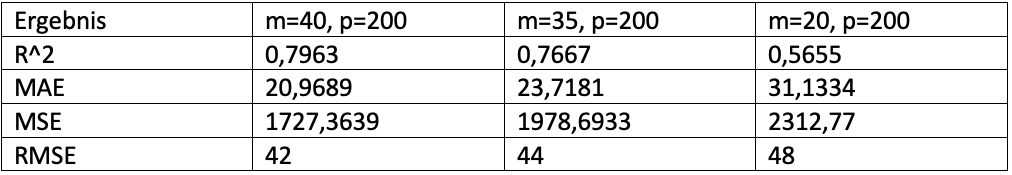
\includegraphics[width=1\textwidth]{Ergebnisse.png}
 \caption{Ergebnistabelle}
\end{figure}

Wie man der Tabelle entnehmen kann, hat man das beste Ergebnis bei \\ n = 40 und p = 200. Der Wert von $R^2$ liegt bei 0,7963 und somit höher als bei den anderen Versuchen. Die MAE, MSE und RMSE Fehler weisen alle einen geringeren Wert auf.
\\\\
Nun werden Originalpreis und vorhergesagter Preis gegenübergestellt.

\begin{figure}[h]
 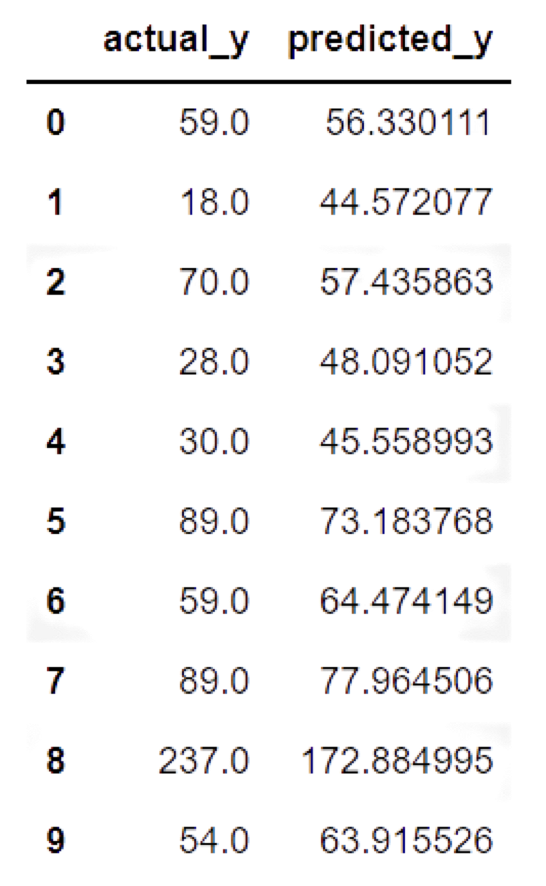
\includegraphics[width=0.3\textwidth]{vergleichpreis.png}
 \caption{Vegleich zwischen Original - und vorhergesagtem Preis}
\end{figure}


Die obenstehende Abbildung zeigt eine Stichprobe des Original Preises pro Nacht (actual\_y) und dem vorhergesagtem Preis (predicted\_y). Für dieses Ergebnis wurde max\_depth = 40 und n\_estimators = 200 gewählt. Wie man sehen kann, gibt es Datensätze, bei denen die Vorhersage gut funktioniert hat ( 0, 2, 6, 7, 9), aber auch einige bei denen die Abweichung größer ausfällt.
\\\\
Jetzt sollen die Merkmale ermittelt werden, die den größten Einfluss auf die Preisbildung haben.
\\
\begin{figure}[h]
 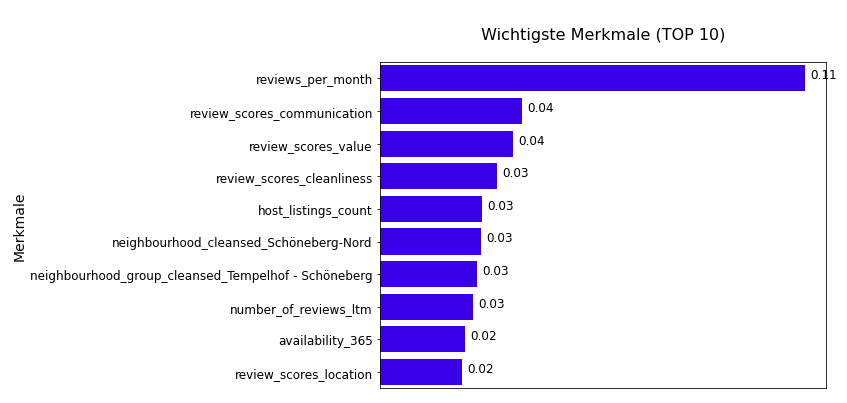
\includegraphics[width=1\textwidth]{wichtigeMermale.png}
 \caption{Auflistung der wichtigsten Mermalen}
\end{figure}
\\
Wie man der Grafik entnehmen kann, hat das Merkmal "review per month" den größten Einfluss auf den Preis. 
\\[0.3 cm]
Darauf folgen "review scores communiction"(Zufriedenheit mit Kommunikation mit Host), "review scores value" (Gesamtbewertung) und "review scores cleanliness" (Zufriedenheit mit Sauberkeitszustand des Angebots).
\\[0.3 cm]
Es fällt auf, dass alle vier, der wichtigsten Merkmale mit der Kundenzufriedenheit zusammen hängen und Merkmale wie die Anzahl der Personen pro Wohnung oder der Ort der Wohnung nicht so einen großen Einfluss auf den Preis haben, wie man vorher vermutet hätte. 
\\[0.3 cm]


\part{Fazit}
Ziel dieses Projektes war es die Immobilienpreisentwicklung in Berlin nachzuvollziehen, einen Preis für ein gegebenes Angebot vorherzusagen und die Merkmale zu ermitteln, die den größten Einfluss auf den Preis haben.\\\\
Die Analysen haben ergeben, dass der Großteil der Airbnb Angebote zentral liegt und es sich vor Allem um Häuser/Wohnungen und private Zimmer handelt.
\\
Der Median ist stadtteilübergreifend sehr konstant, allerdings gibt es bei den zentral gelegenen Bezirken höhere Auspregungen nach oben, als bei den am Rand gelegenen.
\\
Der Durchschnittspreis steigt an, je näher das Wochenende kommt und fällt zum Wochenstart wieder auf den Tiefpunkt.
\\\\
Der Random Forest Algorithmus hat sich als eine geeignete Methode zur Vorhersage der Preise erwiesen. 
\\
Als Merkmale, die den Preis am stärksten beeinflussen, haben sich "Reviews pro Monat", "Bewertung der Kommunikation", "Bewertung der Sauberkeit" und die "Gesamtbewertung" ergeben.
\\\\
Alle vier Merkmale hängen, wie vorher nicht zu erwarten war, sehr stark von der Mieterzufriedenheit ab. Wenn man also seine Wohnung vermieten möchte, sollte man besonders darauf achten, positive Reviews von den Mietern zu erhalten. Das erreicht man am besten, indem man schnell und freundlich auf Anfragen der Mieter antwortet und die Wohnung stets in einem guten Zustand ist.
\newpage
\part{Declaration of Authorship }
\\\\

We hereby confirm that we have authored this Seminar paper independently and without use of others than the indicated sources. All passages (and codes) which are literally or in general matter taken out of publications or other sources are marked as such.
\\\\

Berlin, 27.02.2022, Leander Piepenbring, Minh Anh Le


\newpage
\part * { Literaturverzeichnis }
\addcontentsline{toc}{part}{Literaturverzeichnis}\\\\

\big[1\big] \bfseries\itshape\underline{}{An Introduction to Statistical Learning},\mdseries {https://www.statlearning.com, letzte Stand: 27.02.2022}. \\\\

\big[2\big] \bfseries\itshape\underline{}{Stackabuse},\mdseries {https://stackabuse.com/random-forest-algorithm-with-python-and-scikit-learn/, letzte Stand: 27.02.2022}. \\\\

\big[3\big] \bfseries\itshape\underline{}{Github},\mdseries {https://github.com/Franky007Bond/Airbnb-Munich-Data-Analysis/blob/master/Munich_Airbnb_Data_Analysis.ipynb, letzte Stand: 27.02.2022}. \\\\

\big[4\big] \bfseries\itshape\underline{}{Towards Data Science},\mdseries {https://towardsdatascience.com/predicting-airbnb-prices-in-lisbon-trees-and-random-forests-336d19cdf5a2, letzte Stand: 27.02.2022} \\\\

\big[5\big] \bfseries\itshape\underline{}{Machine Learning Mastery},\mdseries {https://machinelearningmastery.com/random-forest-ensemble-in-python/, letzte Stand: 27.02.2022} \\\\

\big[6\big] \bfseries\itshape\underline{}{Kaggle},\mdseries {https://www.kaggle.com/adityadeshpande23/random-forest-regressor-for-airbnb-rooms-price, letzte Stand: 27.02.2022} \\\\

\big[7\big] \bfseries\itshape\underline{}{Medium},\mdseries {https://medium.com/analytics-vidhya/model-to-predict-booking-prices-on-airbnb-data-science-interview-at-airnbnb-c94675aadec1, letzte Stand: 27.02.2022} \\\\

\big[8\big] \bfseries\itshape\underline{}{Medium},\mdseries {https://medium.com/analytics-vidhya/how-to-analyze-airbnb-performance-data-in-the-right-way-b83f3dad1458, letzte Stand: 27.02.2022} \\\\


\end{text}
\end{document}
